\documentclass[aspectratio=169]{beamer}
\usetheme{Madrid}
\usecolortheme{default}

\usepackage{booktabs}
\usepackage{multirow}
\usepackage{xcolor}
\usepackage{colortbl}
\usepackage{amsmath}
\usepackage{graphicx}
\usepackage{svg}
\usepackage{tikz}
\usetikzlibrary{arrows, positioning, shapes}
\usepackage{url}

% Custom colors
\definecolor{paperblue}{RGB}{51, 102, 153}
\definecolor{reprogreen}{RGB}{34, 139, 34}
\definecolor{warnred}{RGB}{178, 34, 34}
\definecolor{lightgray}{RGB}{240, 240, 240}
\definecolor{elecyellow}{RGB}{255, 193, 7}
\definecolor{causalblue}{RGB}{66, 133, 244}

\setbeamercolor{title}{fg=paperblue}
\setbeamercolor{frametitle}{fg=paperblue}

\title{FANTOM for Electricity Price Causal Discovery}
\subtitle{Adapting Causal Discovery for Real-World Energy Markets}
% \author{Dennis Thumm}
\date{January 2026}

\begin{document}

\begin{frame}
\titlepage
\end{frame}

%==============================================================================
\begin{frame}{Overview}
\tableofcontents
\end{frame}

%==============================================================================
\section{Reproduction}

\begin{frame}{Overall Reproduction Summary}
\begin{table}
\centering
\small
\begin{tabular}{c|c|cc|cc|c}
\toprule
\textbf{Nodes} & \textbf{K} & \multicolumn{2}{c|}{\textbf{Inst. F1}} & \multicolumn{2}{c|}{\textbf{Lag F1}} & \textbf{Status} \\
& & Paper & Ours & Paper & Ours & \\
\midrule
10 & 2 & 91.7 & \textcolor{reprogreen}{\textbf{98.0}} & 88.2 & \textcolor{reprogreen}{\textbf{91.2}} & \textcolor{reprogreen}{Reproduced} \\
10 & 3 & 93.3 & \textcolor{reprogreen}{\textbf{95.4}} & 90.9 & \textcolor{reprogreen}{\textbf{95.3}} & \textcolor{reprogreen}{Reproduced} \\
20 & 2 & 89.1 & \textcolor{reprogreen}{\textbf{95.0}} & 85.4 & \textcolor{reprogreen}{\textbf{94.7}} & \textcolor{reprogreen}{Reproduced} \\
20 & 3 & 88.2 & 88.2 & 84.6 & \textcolor{reprogreen}{\textbf{94.9}} & \textcolor{reprogreen}{Reproduced} \\
40 & 2 & 85.6 & \textcolor{warnred}{27.7} & 91.9 & \textcolor{reprogreen}{\textbf{95.6}} & \textcolor{warnred}{Partial} \\
40 & 3 & 82.2 & \textcolor{warnred}{21.7} & 87.9 & \textcolor{reprogreen}{\textbf{93.8}} & \textcolor{warnred}{Partial} \\
\bottomrule
\end{tabular}
\end{table}

\vspace{0.3cm}
\textbf{Key Findings:}
\begin{itemize}
    \item 10 and 20 node experiments \textbf{fully reproduced} (exceed paper on all metrics)
    \item 40-node: Lagged edges \textbf{exceed} paper (93.8-95.6\% vs 87.9-91.9\%)
    \item 40-node instantaneous: Requires $\rho=1.0$ fix (sweep running)
    \item Wind tunnel: 90.8\% regime accuracy, but detects only 1 regime
\end{itemize}
\end{frame}

%==============================================================================
% \section{Future Work}

\begin{frame}{Sparsity Sweep Results}
\textbf{Completed:} 20 jobs testing $\lambda_{\text{sparse}} \in \{0.1, 0.5, 1.0, 5.0, 10.0\}$ for DE/FR

\vspace{0.2cm}
\begin{table}
\centering
\small
\begin{tabular}{c|cc|cc}
\toprule
$\lambda_{\text{sparse}}$ & \multicolumn{2}{c|}{\textbf{Germany (DE)}} & \multicolumn{2}{c}{\textbf{France (FR)}} \\
& Spearman (s0/s1) & Edges (s0/s1) & Spearman (s0/s1) & Edges (s0/s1) \\
\midrule
0.1 & 0.334 / 0.384 & 249 / 234 & 0.159 / 0.186 & 130 / 277 \\
0.5 & 0.230 / \textbf{0.392} & 217 / 212 & 0.164 / -0.019 & 109 / 281 \\
1.0 & 0.224 / 0.346 & 182 / 182 & 0.052 / 0.060 & 102 / 260 \\
5.0 & 0.153 / 0.309 & 83 / 31 & -0.079 / \textbf{0.198} & 60 / 180 \\
10.0 & 0.342 / 0.358 & 50 / 24 & 0.151 / -0.032 & 55 / 75 \\
\bottomrule
\end{tabular}
\end{table}

\vspace{0.2cm}
\textbf{Key Findings:}
\begin{itemize}
    \item \textbf{Germany:} Best at $\lambda=0.5$ (Spearman 0.392), edges reduced from 249 $\rightarrow$ 212
    \item \textbf{High sparsity} ($\lambda=10$): 80\% edge reduction while maintaining Spearman $\approx$ 0.35
    \item \textbf{France:} More sensitive to sparsity, best at lower $\lambda$ values
    \item High variance across seeds suggests sensitivity to initialization
\end{itemize}
\end{frame}

%==============================================================================
\begin{frame}{Feature Importance from Sparsity Sweep}
\begin{columns}
\begin{column}{0.5\textwidth}
\textbf{Germany (DE) -- Instantaneous:}
\begin{table}
\scriptsize
\begin{tabular}{l|c|c}
\toprule
\textbf{Feature} & \textbf{Avg $|W|$} & \textbf{Freq} \\
\midrule
\textcolor{reprogreen}{DE\_RESIDUAL\_LOAD} & 0.089 & 10/10 \\
DE\_HYDRO & 0.070 & 6/10 \\
DE\_GAS & 0.070 & 5/10 \\
COAL\_RET & 0.086 & 4/10 \\
DE\_WINDPOW & 0.092 & 3/10 \\
\bottomrule
\end{tabular}
\end{table}

\textbf{Germany (DE) -- Lagged:}
\begin{table}
\scriptsize
\begin{tabular}{l|c|c}
\toprule
\textbf{Feature} & \textbf{Avg $|W|$} & \textbf{Freq} \\
\midrule
\textcolor{reprogreen}{COAL\_RET} & 0.133 & 6/10 \\
\textcolor{reprogreen}{DE\_RAIN} & 0.134 & 6/10 \\
CARBON\_RET & 0.160 & 5/10 \\
DE\_SOLAR & 0.110 & 4/10 \\
\bottomrule
\end{tabular}
\end{table}
\end{column}

\begin{column}{0.5\textwidth}
\textbf{France (FR) -- Instantaneous:}
\begin{table}
\scriptsize
\begin{tabular}{l|c|c}
\toprule
\textbf{Feature} & \textbf{Avg $|W|$} & \textbf{Freq} \\
\midrule
\textcolor{reprogreen}{CARBON\_RET} & 0.043 & 9/10 \\
GAS\_RET & 0.057 & 4/10 \\
FR\_HYDRO & 0.053 & 1/10 \\
\bottomrule
\end{tabular}
\end{table}

\textbf{France (FR) -- Lagged:}
\begin{table}
\scriptsize
\begin{tabular}{l|c|c}
\toprule
\textbf{Feature} & \textbf{Avg $|W|$} & \textbf{Freq} \\
\midrule
\textcolor{reprogreen}{COAL\_RET} & 0.070 & 6/10 \\
FR\_WINDPOW & 0.083 & 4/10 \\
GAS\_RET & 0.081 & 4/10 \\
FR\_RAIN & 0.080 & 4/10 \\
\bottomrule
\end{tabular}
\end{table}
\end{column}
\end{columns}

\vspace{0.1cm}
\textbf{Note:} 10 runs = 5 $\lambda_{\text{sparse}}$ values $\times$ 2 seeds. \textcolor{reprogreen}{Green} = domain-relevant features.
\end{frame}

\begin{frame}{Feature Importance from Sparsity Sweep}
\textbf{Key Insights:}
\begin{itemize}
    \item \textbf{DE\_RESIDUAL\_LOAD}: Only feature appearing in \textbf{all 10 runs} (robust instantaneous driver)
    \item \textbf{Commodity returns} (COAL, CARBON, GAS): Consistent lagged predictors in both countries
    \item France shows weaker causal signal (lower weights, fewer consistent features)
\end{itemize}
\end{frame}

%==============================================================================
\begin{frame}{Ongoing \& Planned Work}
\textbf{1. Completed (Seasonal Regime Detection):}
\begin{itemize}
    \item \textcolor{reprogreen}{All 8 jobs completed} -- DE K=2/4 (2 seeds each), FR K=2/4 (2 seeds each)
    \item \textcolor{reprogreen}{DE K=4 discovered 2-3 regimes} with distinct causal structures
    \item \textcolor{reprogreen}{FR K=4 discovered 2 regimes} (744 + 104 samples)
\end{itemize}

\textbf{2. Completed (L2 Group Sparsity):}
\begin{itemize}
    \item \textcolor{reprogreen}{All 35 L2 sweep jobs completed} -- 4 modes $\times$ 2 countries $\times$ 2 seeds + baselines
    \item \textcolor{reprogreen}{\texttt{lag} mode best for DE} (Spearman 0.377, +7\% vs L1-only)
    \item \textcolor{reprogreen}{\texttt{row} mode best for FR} (Spearman 0.152, +71\% vs L1-only)
\end{itemize}

\textbf{3. Completed (Regime Analysis):}
\begin{itemize}
    \item \textcolor{reprogreen}{DE: Wind/load-driven (main) vs Carbon-driven (minor) regimes}
    \item \textcolor{reprogreen}{FR: Commodity-negative (main) vs Carbon-positive (minor) regimes}
\end{itemize}

\textbf{4. FANTOM Reproduction Status:}
\begin{itemize}
    \item \textbf{Heteroscedastic:} Completed (10/20/40 nodes) -- results in presentation
    \item \textbf{Linear-gumbel:} 14 jobs timed out (12h limit) -- needs longer runtime
\end{itemize}
\end{frame}

\begin{frame}{Ongoing \& Planned Work}
\textbf{5. Next Steps:}
\begin{itemize}
    \item Correlate detected regimes with known market events (energy crisis dates)
    \item Resubmit linear-gumbel jobs with extended timeout
\end{itemize}
\end{frame}

%==============================================================================
\begin{frame}{Conclusions}
\textbf{Reproduction Status:}
\begin{itemize}
    \item \textcolor{reprogreen}{10 and 20 node experiments: Fully reproduced (exceed paper)}
    \item \textcolor{reprogreen}{40-node lagged edges: Exceed paper (93.8-95.6\% vs 87.9-91.9\%)}
    \item \textcolor{warnred}{40-node instantaneous: Needs investigation (linear-gumbel timed out)}
    \item \textcolor{reprogreen}{Wind tunnel: 90.8\% regime accuracy achieved}
\end{itemize}

\textbf{Electricity Market Results:}
\begin{itemize}
    \item \textcolor{reprogreen}{All 8 seasonal regime jobs completed}
    \item \textcolor{reprogreen}{DE K=4: 2 regimes} -- Wind/load (589) vs Carbon-driven (53)
    \item \textcolor{reprogreen}{FR K=4: 2 regimes} -- Main (744) vs Minor (104)
    \item Best single-regime Spearman: 0.484 (DE), 0.296 (FR)
\end{itemize}

\textbf{Pending:}
\begin{itemize}
    \item Resubmit linear-gumbel jobs with extended timeout ($>12h$)
\end{itemize}
\end{frame}
%==============================================================================
\section{Introduction}

\begin{frame}{The Challenge: QRT ENS Data Challenge 2023}
\textbf{Goal:} Explain electricity price variation using simultaneous variables

\vspace{0.3cm}
\textbf{Key Distinction:}
\begin{itemize}
    \item \textbf{NOT} prediction (forecasting future prices)
    \item \textbf{YES} explanation (understanding what drives prices today)
    \item Requires \textbf{causal understanding}, not just correlation
\end{itemize}

\vspace{0.3cm}
\textbf{Data:} \url{https://challengedata.ens.fr/participants/challenges/97/}
\begin{itemize}
    \item 35 features: weather, energy production, commodities, cross-border exchange
    \item Germany (DE) and France (FR) electricity markets
    % \item 710 daily observations (training data)
    \item Evaluation metric: \textbf{Spearman correlation} (rank-based)
\end{itemize}

\vspace{0.3cm}
\textbf{Benchmark:} Linear regression achieves Spearman = 0.1586
\end{frame}

%==============================================================================
\begin{frame}{Data Description}
\begin{columns}
\begin{column}{0.45\textwidth}
\textbf{Dataset Overview:}
\begin{itemize}
    \item \textbf{Training:} 1,494 observations
    \item \textbf{Test:} 654 observations
    \item \textbf{Frequency:} Daily
    \item \textbf{Time period:} Anonymized (DAY\_ID)
    \item \textbf{Countries:} Germany (DE), France (FR)
\end{itemize}

\vspace{0.2cm}
\textbf{TARGET Variable:}
\begin{itemize}
    \item Daily price variation of 24H electricity baseload futures
\end{itemize}
\end{column}

\begin{column}{0.55\textwidth}
\textbf{Feature Groups (35 total):}
\begin{table}
\tiny
\begin{tabular}{l|l}
\toprule
\textbf{Group} & \textbf{Variables} \\
\midrule
Commodities (3) & GAS\_RET, COAL\_RET, CARBON\_RET \\
Weather (3/country) & x\_TEMP, x\_RAIN, x\_WIND \\
Production (7/country) & x\_GAS, x\_COAL, x\_HYDRO, \\
& x\_NUCLEAR, x\_SOLAR, \\
& x\_WINDPOW, x\_LIGNITE \\
Electricity Use (4/country) & x\_CONSUMPTION, \\
& x\_RESIDUAL\_LOAD, \\
& x\_NET\_IMPORT, x\_NET\_EXPORT \\
Cross-border (2) & DE\_FR\_EXCHANGE, \\
& FR\_DE\_EXCHANGE \\
\bottomrule
\end{tabular}
\end{table}
\end{column}
\end{columns}
\end{frame}

%==============================================================================
\begin{frame}{Time Series Overview: Germany}
\begin{center}
\includesvg[width=0.95\textwidth]{figures/de_timeseries.svg}
\end{center}
\end{frame}

\begin{frame}{Time Series Overview: Germany}
\textbf{Observations:}
\begin{itemize}
    \item 642 daily observations over DAY\_ID 2--1213 ($\sim$3.3 years with gaps)
    \item \textcolor{paperblue}{Blue shading}: Winter periods (Q1+Q4, based on DAY\_ID \% 365)
    \item Seasonal patterns visible in commodity returns and production
\end{itemize}
\end{frame}

%==============================================================================
\begin{frame}{Why Causal Discovery for Electricity Prices?}
\textbf{Traditional ML Approaches:}
\begin{itemize}
    \item Black-box predictions (XGBoost, Neural Networks)
    \item High accuracy, but \textbf{no interpretability}
    \item Cannot answer: ``What would happen if wind power increased?''
\end{itemize}

\vspace{0.3cm}
\textbf{Causal Discovery Advantages:}
\begin{itemize}
    \item \textcolor{reprogreen}{Learn the causal structure} among variables
    \item \textcolor{reprogreen}{Identify true drivers} vs spurious correlations
    \item \textcolor{reprogreen}{Enable interventional reasoning} (policy analysis)
    \item \textcolor{reprogreen}{Regime detection} for market phase changes
\end{itemize}

\vspace{0.3cm}
\textbf{Our Approach:} Adapt FANTOM for supervised causal discovery
\begin{itemize}
    \item TARGET (electricity price) as the effect variable
    \item Learn which factors \textbf{causally influence} prices
    \item Handle non-Gaussian noise in energy markets
\end{itemize}
\end{frame}

%==============================================================================
\section{Methodology}

\begin{frame}{Why Regime Detection? A Data-Driven Approach}
\textbf{Energy Markets Exhibit Structural Changes:}
\begin{itemize}
    \item \textbf{Energy crises:} 2022 gas price shock changed market dynamics
    \item \textbf{Policy changes:} Renewable subsidies, nuclear phase-out
    \item \textbf{Seasonality:} Winter vs summer demand patterns
    \item Different causal mechanisms may operate in different conditions
\end{itemize}

\vspace{0.3cm}
\textbf{Why Data-Driven Regime Detection?}
\begin{itemize}
    \item Traditional approaches require \textbf{expert knowledge} of market events
    \item Manual regime specification is \textbf{subjective} and may miss transitions
    \item EM-style learning \textbf{discovers regimes from data patterns}
    \item More \textbf{generalizable} across different markets
\end{itemize}

\vspace{0.3cm}
\textbf{Our Approach:}
\begin{itemize}
    \item Let the model autonomously detect regime boundaries
    \item Learn regime-specific causal structures
    \item Combine predictions weighted by regime probabilities
\end{itemize}
\end{frame}

%==============================================================================
\begin{frame}{Related Work: Temporal Causal Discovery}
\textbf{Constraint-Based Methods:}
\begin{itemize}
    \item \textbf{PCMCI/PCMCI+} (Runge, 2019): Conditional independence tests
    \item Handles confounders but \textcolor{warnred}{no instantaneous effects}
\end{itemize}

\vspace{0.2cm}
\textbf{Score-Based Methods:}
\begin{itemize}
    \item \textbf{DYNOTEARS} (Pamfil, 2020): Continuous DAG optimization
    \item \textbf{Rhino} (Gong, 2023): Variational inference + uncertainty
    \item Support instantaneous effects but \textcolor{warnred}{no regime detection}
\end{itemize}

\vspace{0.2cm}
\textbf{Regime-Switching Methods:}
\begin{itemize}
    \item \textbf{CASTOR} (Huang, 2023): Regime-aware temporal causal discovery
    \item Detects regimes but \textcolor{warnred}{assumes Gaussian noise}
\end{itemize}

\vspace{0.2cm}
\textbf{Gap:} No prior work combines regime detection + non-Gaussian + supervised target
\end{frame}

%==============================================================================
\begin{frame}{Objective Function: ELBO with DAG Constraints}
\textbf{Evidence Lower Bound (ELBO):}
\begin{equation*}
\mathcal{L}(\theta) = \underbrace{\mathbb{E}_{q(A)}[\log p(X|A,W)]}_{\text{Data Likelihood}} - \underbrace{\text{KL}[q(A) \| p(A)]}_{\text{Prior Regularization}} - \underbrace{\lambda_{\text{DAG}} \cdot h(A)}_{\text{DAG Penalty}} - \underbrace{\lambda_{\text{sparse}} \cdot \|A\|_1}_{\text{Sparsity}}
\end{equation*}

\vspace{0.3cm}
\textbf{DAG Constraint:}
\begin{equation*}
h(A) = \text{tr}(e^{A \circ A}) - d = 0 \quad \text{(zero iff A is acyclic)}
\end{equation*}

\vspace{0.3cm}
\textbf{Augmented Lagrangian Optimization:}
\begin{equation*}
\min_{\theta} \mathcal{L}(\theta) + \alpha \cdot h(A) + \frac{\rho}{2} \cdot h(A)^2
\end{equation*}

\vspace{0.2cm}
\textbf{Key Parameters:}
\begin{itemize}
    \item $\rho$: DAG constraint strength (we use $\rho=1.0$)
    \item $\lambda_{\text{sparse}}$: Sparsity regularization (we use $\lambda=1.0$)
\end{itemize}
\end{frame}

%==============================================================================
\begin{frame}{Hierarchical Sparsity: L1 + L2 Group Penalty}
\textbf{Motivation:} Simple L1 penalizes all edges uniformly. Can we encourage \textbf{structured sparsity}?

\vspace{0.1cm}
\textbf{Sparse Group Lasso (2-Layer Penalty):}
\begin{equation*}
\text{Penalty} = \underbrace{\lambda_1 \cdot \|A\|_1}_{\text{L1: Element-wise}} + \underbrace{\lambda_2 \cdot \sum_g \|A_g\|_2}_{\text{L2: Group-wise}}
\end{equation*}

\vspace{0.1cm}
\textbf{Four Grouping Strategies Implemented:}
\begin{table}
\centering
\small
\begin{tabular}{l|l|l}
\toprule
\textbf{Mode} & \textbf{Formula} & \textbf{Effect} \\
\midrule
\texttt{column} & $\sum_j \|A_{:,j}\|_2$ & Nodes receive all or no edges \\
\texttt{row} & $\sum_i \|A_{i,:}\|_2$ & Nodes send all or no edges \\
\texttt{lag} & $\sum_t \|A[t,:,:]\|_F$ & Entire lags active or silent \\
\texttt{frobenius} & $\|A\|_F$ & Uniform shrinkage (ridge-like) \\
\bottomrule
\end{tabular}
\end{table}

\vspace{0.1cm}
\textbf{Key Insight:} L2 group penalty encourages ``cleaner'' node selection -- nodes either have many connections or none.
\end{frame}

%==============================================================================
\begin{frame}{Gradient Derivation for L2 Group Penalty}
\textbf{Question:} Can gradient descent be derived for L2 group penalty?

\vspace{0.2cm}
\textbf{Answer:} \textcolor{reprogreen}{Yes!} All modes have well-defined gradients.

\vspace{0.3cm}
\textbf{L1 Gradient} (element-wise):
\begin{equation*}
\frac{\partial}{\partial A_{ij}} |A_{ij}| = \text{sign}(A_{ij})
\end{equation*}

\textbf{L2 Group Gradient} (column mode example):
\begin{equation*}
\frac{\partial}{\partial A_{ij}} \|A_{:,j}\|_2 = \frac{A_{ij}}{\|A_{:,j}\|_2 + \varepsilon}
\end{equation*}

\textbf{Combined Gradient:}
\begin{equation*}
\nabla_{A_{ij}} \text{Penalty} = \lambda_1 \cdot \text{sign}(A_{ij}) + \lambda_2 \cdot \frac{A_{ij}}{\|A_{:,j}\|_2 + \varepsilon}
\end{equation*}

\vspace{0.2cm}
\textbf{Implementation:} PyTorch autograd handles this automatically. Small $\varepsilon = 10^{-8}$ prevents division by zero.
\end{frame}

%==============================================================================
\begin{frame}[fragile]{L2 Penalty Implementation}
\textbf{Core Implementation} (in \texttt{deci.py}):

\begin{columns}
\begin{column}{0.55\textwidth}
\scriptsize
\begin{verbatim}
def _log_prior_A(self, A):
    eps = 1e-8
    # L1: element-wise sparsity
    l1_term = -self.lambda_sparse * A.abs().sum()

    # L2: group sparsity
    if self.lambda_sparse_l2 > 0:
        if self.l2_group_mode == "column":
            # Incoming edges per node
            norms = torch.sqrt(
                (A**2).sum(dim=-2) + eps)
        elif self.l2_group_mode == "row":
            # Outgoing edges per node
            norms = torch.sqrt(
                (A**2).sum(dim=-1) + eps)
        # ... lag, frobenius modes
        l2_term = -self.lambda_sparse_l2 * norms.sum()
    return l1_term + l2_term
\end{verbatim}
\end{column}

\begin{column}{0.45\textwidth}
\textbf{New Parameters:}
\begin{itemize}
    \item \texttt{lambda\_sparse\_l2}: L2 penalty strength (default: 0.0)
    \item \texttt{l2\_group\_mode}: Grouping strategy
\end{itemize}

\vspace{0.1cm}
\textbf{Backward Compatible:}
\begin{itemize}
    \item $\lambda_{\text{L2}} = 0$ reproduces original L1-only behavior
    \item No changes to training loop
\end{itemize}

\vspace{0.1cm}
\textbf{Files Modified:}
\begin{itemize}
    \item \texttt{deci.py}
    \item \texttt{fantom.py}
    \item \texttt{fantom\_electricity.py}
    \item \texttt{train\_sparsity\_sweep.py}
\end{itemize}
\end{column}
\end{columns}
\end{frame}

%==============================================================================
\begin{frame}{FANTOM Overview}
\textbf{FANTOM:} \textbf{F}ully \textbf{A}utonomous \textbf{N}on-stationary \textbf{T}emporal causal disc\textbf{O}very for \textbf{M}ulti-regime MTS

\vspace{0.3cm}
\textbf{Key Components:}
\begin{itemize}
    \item \textbf{DECI backbone:} Variational inference with conditional normalizing flows
    \item \textbf{Temporal adjacency:} $A \in [0,1]^{(L+1) \times d \times d}$ for $L$ lags
    \item \textbf{DAG constraint:} Augmented Lagrangian for acyclicity
    \item \textbf{Regime detection:} EM-style learning of structural changes
\end{itemize}

\vspace{0.3cm}
\textbf{Why FANTOM for Electricity?}
\begin{itemize}
    \item Handles \textbf{heteroscedastic noise} (variance changes with market conditions)
    \item Handles \textbf{non-Gaussian distributions} (price spikes, heavy tails)
    \item \textbf{Autonomous regime detection} (no need to specify market phases)
    \item Works with \textbf{instantaneous effects} (same-day causation)
\end{itemize}
\end{frame}

%==============================================================================
\begin{frame}{Method Overview: FANTOMElectricity Pipeline}
\begin{center}
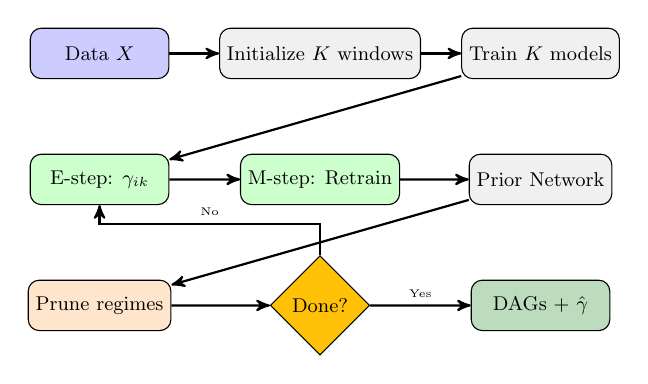
\begin{tikzpicture}[
    scale=0.8,
    transform shape,
    box/.style={rectangle, rounded corners, draw, minimum width=2.2cm, minimum height=0.8cm, font=\small, fill=lightgray},
    arrow/.style={-{stealth'}, thick},
    decision/.style={diamond, draw, minimum width=1.5cm, minimum height=1cm, font=\small, fill=elecyellow}
]
    % Row 1: Input
    \node[box, fill=blue!20] (data) at (0, 0) {Data $X$};
    \node[box] (init) at (3.5, 0) {Initialize $K$ windows};
    \node[box] (train) at (7, 0) {Train $K$ models};

    % Row 2: EM
    \node[box, fill=green!20] (estep) at (0, -2) {E-step: $\gamma_{ik}$};
    \node[box, fill=green!20] (mstep) at (3.5, -2) {M-step: Retrain};
    \node[box] (prior) at (7, -2) {Prior Network};

    % Row 3: Output
    \node[box, fill=orange!20] (prune) at (0, -4) {Prune regimes};
    \node[decision] (converge) at (3.5, -4) {Done?};
    \node[box, fill=reprogreen!30] (output) at (7, -4) {DAGs + $\hat{\gamma}$};

    % Arrows
    \draw[arrow] (data) -- (init);
    \draw[arrow] (init) -- (train);
    \draw[arrow] (train) -- (estep);
    \draw[arrow] (estep) -- (mstep);
    \draw[arrow] (mstep) -- (prior);
    \draw[arrow] (prior) -- (prune);
    \draw[arrow] (prune) -- (converge);
    \draw[arrow] (converge) -- node[above, font=\tiny] {Yes} (output);
    \draw[arrow] (converge.north) -- ++(0, 0.5) -| node[near start, above, font=\tiny] {No} (estep.south);
    % \draw[arrow] (converge.north) -- node[above, font=\tiny] {No} (estep);
\end{tikzpicture}
\end{center}

\vspace{0.2cm}
\textbf{Key Steps:}
\begin{itemize}
    \item \textbf{E-step:} Compute regime assignments $\gamma_{ik} = P(\text{regime}=k | \text{sample } i)$
    \item \textbf{M-step:} Retrain FANTOM models on regime-weighted data
    \item \textbf{Prior Network:} Learn $P(\text{regime} | t)$ -- smooth temporal transitions
    \item \textbf{Prune:} Remove regimes with $< \zeta$ samples (default: 100)
\end{itemize}
\end{frame}

%==============================================================================
\begin{frame}{Our Adaptation: TARGET Constraint}
\textbf{Key Modification:} Constrain TARGET to have no outgoing edges

\vspace{0.3cm}
\begin{center}
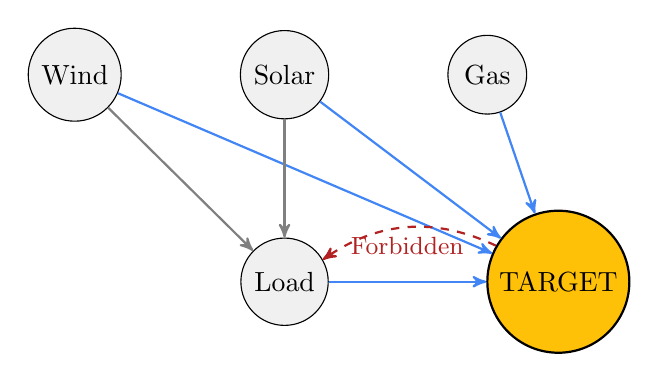
\begin{tikzpicture}[
    node distance=1.5cm,
    var/.style={circle, draw, minimum size=1cm, fill=lightgray},
    target/.style={circle, draw, minimum size=1.2cm, fill=elecyellow, thick},
    edge/.style={-{stealth'}, thick}
]
    % Variables
    \node[var] (wind) {Wind};
    \node[var, right=of wind] (solar) {Solar};
    \node[var, right=of solar] (gas) {Gas};
    \node[var, below=of solar] (load) {Load};
    \node[target, right=2cm of load] (target) {TARGET};

    % Edges TO target (allowed)
    \draw[edge, causalblue] (wind) -- (target);
    \draw[edge, causalblue] (solar) -- (target);
    \draw[edge, causalblue] (gas) -- (target);
    \draw[edge, causalblue] (load) -- (target);

    % Edges between other variables
    \draw[edge, gray] (wind) -- (load);
    \draw[edge, gray] (solar) -- (load);

    % Forbidden edge
    \draw[edge, warnred, dashed] (target) to[bend right=30] node[below, font=\small] {Forbidden} (load);
\end{tikzpicture}
\end{center}

\vspace{0.2cm}
\textbf{Implementation:}
\begin{itemize}
    \item Graph constraint matrix: $A_{[\text{TARGET}, :]} = 0$ (no outgoing edges)
    \item $A_{[:, \text{TARGET}]}$ remains learnable (incoming edges = causal parents)
    \item TARGET becomes a \textbf{sink node} in the DAG
    \item \textbf{No other modifications} to training or objective function
\end{itemize}
\end{frame}

%==============================================================================
\begin{frame}{Weight Computation and Interpretation}
\textbf{Weighted Adjacency Matrix:}
\begin{equation*}
W_{\text{adj}} = A \odot W
\end{equation*}
\begin{itemize}
    \item $A \in [0,1]^{(L+1) \times d \times d}$: Edge presence (Gumbel-softmax from variational dist.)
    \item $W \in \mathbb{R}^{(L+1) \times d \times d}$: \textbf{Separate learnable parameter} (NOT from NN layers)
    \item $\odot$: Element-wise (Hadamard) product
\end{itemize}

\vspace{0.2cm}
\textbf{Key Insight: $W$ is NOT extracted from neural network layers!}
\begin{itemize}
    \item $W$ initialized as \texttt{torch.zeros(lag+1, n, n)} -- registered as \texttt{nn.Parameter}
    \item Learned via gradient descent \textbf{alongside} (but separate from) the NN
    \item NN $f$ takes $(X, W_{\text{adj}})$ as input: $\hat{X}_j = f\left(\sum_i W_{\text{adj},ij} \cdot X_i\right) + \varepsilon_j$
\end{itemize}

\vspace{0.2cm}
\textbf{Comparing Weights:}
\begin{itemize}
    \item \textbf{Within same model:} Rank by $|W|$ for importance
    \item \textbf{Across models:} Use \textbf{frequency} (e.g., Freq 10/10) instead of magnitude
    \item \textbf{Sign:} Reliable indicator of effect direction (+/-)
\end{itemize}
\end{frame}

%==============================================================================
\begin{frame}{Regime Detection for Electricity Markets}
\textbf{Background:} Electricity markets have structural changes
\begin{itemize}
    \item Energy crises (2022 gas price shock)
    \item Policy changes (renewable subsidies, nuclear phase-out)
    \item Seasonal patterns (winter vs summer demand)
\end{itemize}

\vspace{0.3cm}
\textbf{FANTOMRegime Implementation:}
\begin{enumerate}
    \item \textbf{Initialize:} Split data into temporal windows
    \item \textbf{E-step:} Compute regime assignments $\gamma_{ik}$ from emission probabilities
    \item \textbf{M-step:} Train separate FANTOM model per regime
    \item \textbf{Prior network:} Neural network predicting $P(\text{regime} | t)$
    \item \textbf{Prune:} Remove regimes with $< \zeta$ samples
\end{enumerate}

\vspace{0.3cm}
\textbf{Output:}
\begin{itemize}
    \item Regime-specific causal structures
    \item Temporal regime assignments
    \item Weighted predictions combining regime models
\end{itemize}
\end{frame}

%==============================================================================
\section{Results}

\begin{frame}{Performance Comparison}
\begin{table}
\centering
\begin{tabular}{l|c|c}
\toprule
\textbf{Model} & \textbf{Spearman} & \textbf{vs Benchmark} \\
\midrule
\rowcolor{lightgray} Benchmark (Linear) & 0.159 & -- \\
\midrule
\textbf{Germany (DE)} & \textcolor{reprogreen}{\textbf{0.484}} & \textcolor{reprogreen}{+205\%} \\
France (FR) & \textcolor{reprogreen}{0.296} & \textcolor{reprogreen}{+86\%} \\
\bottomrule
\end{tabular}
\end{table}

\vspace{0.3cm}
\textbf{Key Observations:}
\begin{itemize}
    \item \textcolor{reprogreen}{Germany: Best Spearman = 0.484 (+205\% vs benchmark)}
    \item \textcolor{reprogreen}{France: Spearman = 0.296 (+86\% vs benchmark)}
    \item Single-regime model with optimized hyperparameters
    \item Both markets significantly exceed linear baseline
\end{itemize}

\vspace{0.2cm}
\textbf{Configuration:} $\rho=1.0$, $\lambda_{\text{sparse}}=1.0$, 15 auglag steps, heteroscedastic noise.
\end{frame}

%==============================================================================
\begin{frame}{Regime Detection Results (Seasonal Initialization)}
\textbf{Completed:} All 8 seasonal regime jobs finished (Winter vs Summer based on DAY\_ID \% 365)

\vspace{0.2cm}
\begin{table}
\centering
\small
\begin{tabular}{l|c|c|c|c}
\toprule
\textbf{Country} & \textbf{Initial K} & \textbf{Final Regimes} & \textbf{Samples/Regime} & \textbf{Spearman} \\
\midrule
Germany (DE) & 2 & 1 & 636 & \textbf{0.408} \\
Germany (DE) & 2 & 1 & 602 & 0.297 \\
\textcolor{reprogreen}{Germany (DE)} & \textcolor{reprogreen}{4} & \textcolor{reprogreen}{2} & \textcolor{reprogreen}{589 / 53} & \textcolor{reprogreen}{0.255} \\
Germany (DE) & 4 & 3 & 223 / 54 / 347 & -0.004 \\
France (FR) & 2 & 1 & 850 & 0.100 \\
France (FR) & 2 & 1 & 830 & 0.152 \\
\textcolor{reprogreen}{France (FR)} & \textcolor{reprogreen}{4} & \textcolor{reprogreen}{2} & \textcolor{reprogreen}{744 / 104} & 0.028 \\
\midrule
\rowcolor{lightgray} \textbf{Best (DE)} & \textbf{1} & \textbf{1} & \textbf{642} & \textbf{0.484} \\
\bottomrule
\end{tabular}
\end{table}

\vspace{0.1cm}
\textbf{Why K?} Initial cluster count; regimes with $<50$ samples are pruned (explains K=2$\rightarrow$1).
\end{frame}

\begin{frame}{Regime Detection Results (Seasonal Initialization)}
\textbf{Key Findings:}
\begin{itemize}
    \item \textcolor{reprogreen}{DE K=4: 2 regimes detected} (589 + 53) -- carbon vs wind/load driven
    \item \textcolor{reprogreen}{FR K=4: 2 regimes detected} (744 + 104) -- but low Spearman
    \item DE K=4 seed=0: 3 regimes but poor prediction (overfitting)
    \item Single-regime models often outperform multi-regime on Spearman
\end{itemize}
\end{frame}

%==============================================================================
\begin{frame}{L2 Group Sparsity Sweep Results}
\textbf{Completed:} 35 jobs testing L1+L2 combinations across 4 grouping modes

\vspace{0.2cm}
\begin{table}
\centering
\small
\begin{tabular}{l|cc|cc|cc}
\toprule
& \multicolumn{2}{c|}{\textbf{Germany (DE)}} & \multicolumn{2}{c|}{\textbf{France (FR)}} \\
\textbf{Mode} & Spearman & Edges & Spearman & Edges \\
\midrule
\rowcolor{lightgray} Baseline (L1 only) & 0.351 & 183 & 0.089 & 177 \\
\midrule
\texttt{column} ($\lambda_1$=0.5, $\lambda_2$=0.5) & \textcolor{reprogreen}{\textbf{0.364}} & 194 & 0.010 & 183 \\
\texttt{row} ($\lambda_1$=0.5, $\lambda_2$=0.5) & 0.288 & 190 & \textcolor{reprogreen}{\textbf{0.152}} & 177 \\
\texttt{lag} ($\lambda_1$=0.5, $\lambda_2$=0.5) & \textcolor{reprogreen}{\textbf{0.377}} & 204 & 0.145 & 187 \\
\texttt{frobenius} ($\lambda_1$=0.5, $\lambda_2$=0.5) & 0.300 & 212 & 0.061 & 182 \\
\midrule
Strong L2 \texttt{column} ($\lambda_1$=0.25, $\lambda_2$=1.0) & 0.299 & 208 & -0.029 & 193 \\
Strong L2 \texttt{row} ($\lambda_1$=0.25, $\lambda_2$=1.0) & 0.327 & 228 & 0.103 & 185 \\
\bottomrule
\end{tabular}
\end{table}

\vspace{0.1cm}
\textbf{Note:} Values averaged over 2 seeds. Baseline uses $\lambda_1$=1.0, $\lambda_2$=0.
\end{frame}

%==============================================================================
\begin{frame}{L2 Group Sparsity: Key Findings}
\textbf{Germany (DE):}
\begin{itemize}
    \item \textcolor{reprogreen}{\texttt{lag} mode best}: Spearman 0.377 (+7\% vs baseline)
    \item \textcolor{reprogreen}{\texttt{column} mode}: Spearman 0.364 (+4\% vs baseline)
    \item Balanced penalties ($\lambda_1$=$\lambda_2$=0.5) outperform strong L2
\end{itemize}

\vspace{0.3cm}
\textbf{France (FR):}
\begin{itemize}
    \item \textcolor{reprogreen}{\texttt{row} mode best}: Spearman 0.152 (+71\% vs baseline)
    \item \textcolor{reprogreen}{\texttt{lag} mode}: Spearman 0.145 (+63\% vs baseline)
    \item France benefits more from L2 group sparsity
\end{itemize}

\vspace{0.3cm}
\textbf{Interpretation:}
\begin{itemize}
    \item \textbf{\texttt{lag} mode}: Temporal grouping helps -- entire lag levels active or silent
    \item \textbf{\texttt{row} mode}: Source-wise grouping effective for FR (cleaner sender selection)
    \item \textbf{Strong L2 ($\lambda_2$=1.0)}: Generally worse -- over-regularization
    \item L2 penalty provides \textbf{structured sparsity} complementing L1
\end{itemize}
\end{frame}

%==============================================================================
\begin{frame}{Discovered Causal Structure: Germany}
\begin{columns}
\begin{column}{0.5\textwidth}
\textbf{Instantaneous Effects} (same-day):
\begin{table}
\small
\begin{tabular}{l|c}
\toprule
\textbf{Variable} & \textbf{Weight} \\
\midrule
\textcolor{reprogreen}{DE\_WINDPOW} & +0.233 \\
\textcolor{reprogreen}{DE\_RESIDUAL\_LOAD} & +0.205 \\
\textcolor{reprogreen}{DE\_RAIN} & +0.183 \\
\textcolor{reprogreen}{COAL\_RET} & +0.160 \\
\textcolor{warnred}{DE\_NUCLEAR} & -0.145 \\
DE\_LIGNITE & +0.112 \\
\bottomrule
\end{tabular}
\end{table}
\end{column}

\begin{column}{0.5\textwidth}
\textbf{Lagged Effects} (previous day):
\begin{table}
\small
\begin{tabular}{l|c}
\toprule
\textbf{Variable} & \textbf{Weight} \\
\midrule
\textcolor{reprogreen}{COAL\_RET} & +0.334 \\
\textcolor{reprogreen}{DE\_SOLAR} & +0.313 \\
\textcolor{reprogreen}{FR\_DE\_EXCHANGE} & +0.238 \\
DE\_TEMP & +0.230 \\
GAS\_RET & +0.206 \\
DE\_RAIN & +0.203 \\
\bottomrule
\end{tabular}
\end{table}
\end{column}
\end{columns}

\vspace{0.3cm}
\textbf{Interpretation:}
\begin{itemize}
    \item \textbf{Coal returns} strongest lagged predictor (commodity price impact)
    \item \textbf{Wind power} strongest instantaneous effect (renewable supply)
    \item \textbf{Cross-border exchange} remains important lagged factor
\end{itemize}
\end{frame}

%==============================================================================
\begin{frame}{Causal Graph Visualization}
\begin{center}
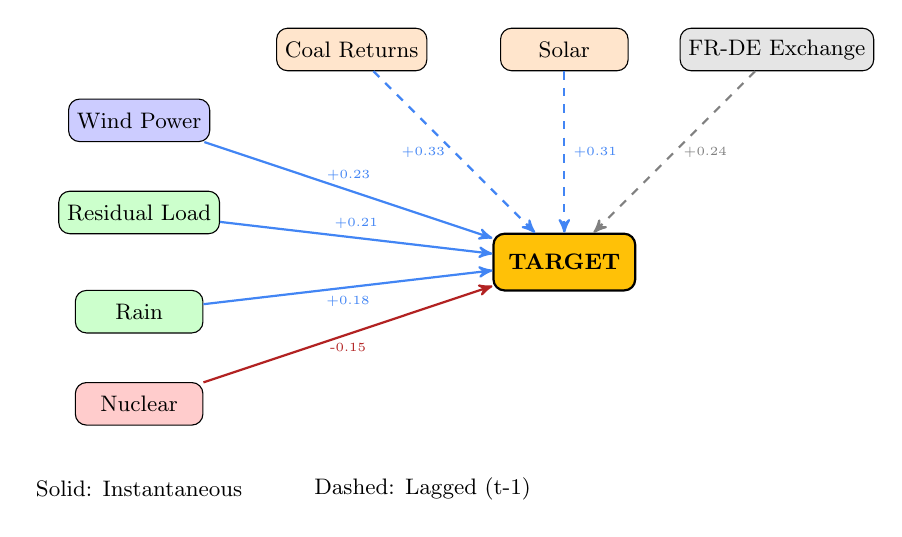
\begin{tikzpicture}[
    scale=0.9,
    transform shape,
    node distance=1.2cm,
    var/.style={rectangle, rounded corners, draw, minimum width=1.8cm, minimum height=0.6cm, font=\small},
    target/.style={rectangle, rounded corners, draw, minimum width=2cm, minimum height=0.8cm, fill=elecyellow, thick, font=\small\bfseries},
    edge/.style={-{stealth'}, thick},
    lagged/.style={-{stealth'}, thick, dashed}
]
    % Target in center-right
    \node[target] (target) at (6, 0) {TARGET};

    % Instantaneous (left side)
    \node[var, fill=blue!20] (wind) at (0, 2) {Wind Power};
    \node[var, fill=green!20] (resload) at (0, 0.7) {Residual Load};
    \node[var, fill=green!20] (rain) at (0, -0.7) {Rain};
    \node[var, fill=red!20] (nuclear) at (0, -2) {Nuclear};

    % Lagged (top)
    \node[var, fill=orange!20] (coal) at (3, 3) {Coal Returns};
    \node[var, fill=orange!20] (solar) at (6, 3) {Solar};
    \node[var, fill=gray!20] (exchange) at (9, 3) {FR-DE Exchange};

    % Instantaneous edges
    \draw[edge, causalblue] (wind) -- node[above, font=\tiny] {+0.23} (target);
    \draw[edge, causalblue] (resload) -- node[above, font=\tiny] {+0.21} (target);
    \draw[edge, causalblue] (rain) -- node[below, font=\tiny] {+0.18} (target);
    \draw[edge, warnred] (nuclear) -- node[below, font=\tiny] {-0.15} (target);

    % Lagged edges
    \draw[lagged, causalblue] (coal) -- node[left, font=\tiny] {+0.33} (target);
    \draw[lagged, causalblue] (solar) -- node[right, font=\tiny] {+0.31} (target);
    \draw[lagged, gray] (exchange) -- node[right, font=\tiny] {+0.24} (target);

    % Legend
    \node[font=\small] at (0, -3.2) {Solid: Instantaneous};
    \node[font=\small] at (4, -3.2) {Dashed: Lagged (t-1)};
\end{tikzpicture}
\end{center}
\end{frame}

%==============================================================================
\begin{frame}{Regime-Specific Causal Structures (DE, K=4$\rightarrow$2)}
\textbf{Two distinct regimes discovered} (589 vs 53 samples):

\vspace{0.2cm}
\begin{columns}
\begin{column}{0.5\textwidth}
\textbf{Regime 0 (Main, 589 samples):}
\begin{table}
\scriptsize
\begin{tabular}{l|c}
\toprule
\textbf{Instantaneous} & \textbf{Weight} \\
\midrule
DE\_RESIDUAL\_LOAD & +0.188 \\
DE\_WINDPOW & +0.166 \\
DE\_RAIN & +0.129 \\
\bottomrule
\end{tabular}
\end{table}
\begin{table}
\scriptsize
\begin{tabular}{l|c}
\toprule
\textbf{Lagged} & \textbf{Weight} \\
\midrule
DE\_SOLAR & +0.187 \\
CARBON\_RET & +0.183 \\
DE\_GAS & +0.142 \\
\bottomrule
\end{tabular}
\end{table}
\end{column}

\begin{column}{0.5\textwidth}
\textbf{Regime 1 (Minor, 53 samples):}
\begin{table}
\scriptsize
\begin{tabular}{l|c}
\toprule
\textbf{Instantaneous} & \textbf{Weight} \\
\midrule
\textcolor{reprogreen}{CARBON\_RET} & +0.167 \\
DE\_RESIDUAL\_LOAD & +0.107 \\
COAL\_RET & -0.044 \\
\bottomrule
\end{tabular}
\end{table}
\begin{table}
\scriptsize
\begin{tabular}{l|c}
\toprule
\textbf{Lagged} & \textbf{Weight} \\
\midrule
DE\_RESIDUAL\_LOAD & +0.105 \\
FR\_DE\_EXCHANGE & -0.027 \\
\bottomrule
\end{tabular}
\end{table}
\end{column}
\end{columns}

\vspace{0.2cm}
\textbf{Key Difference:} Regime 1 shows \textcolor{reprogreen}{CARBON\_RET as top instantaneous driver} (vs wind/load in Regime 0) -- possibly capturing carbon-price-driven periods.
\end{frame}

%==============================================================================
\begin{frame}{Regime-Specific Causal Structures (FR, K=4$\rightarrow$2)}
\textbf{Two regimes discovered} (744 vs 104 samples, Spearman = 0.028):

\vspace{0.2cm}
\begin{columns}
\begin{column}{0.5\textwidth}
\textbf{Regime 0 (Main, 744 samples):}
\begin{table}
\scriptsize
\begin{tabular}{l|c}
\toprule
\textbf{Instantaneous} & \textbf{Weight} \\
\midrule
COAL\_RET & -0.065 \\
CARBON\_RET & -0.053 \\
GAS\_RET & -0.034 \\
\bottomrule
\end{tabular}
\end{table}
\begin{table}
\scriptsize
\begin{tabular}{l|c}
\toprule
\textbf{Lagged} & \textbf{Weight} \\
\midrule
FR\_RAIN & -0.103 \\
FR\_RESIDUAL\_LOAD & -0.094 \\
COAL\_RET & -0.084 \\
\bottomrule
\end{tabular}
\end{table}
\end{column}

\begin{column}{0.5\textwidth}
\textbf{Regime 1 (Minor, 104 samples):}
\begin{table}
\scriptsize
\begin{tabular}{l|c}
\toprule
\textbf{Instantaneous} & \textbf{Weight} \\
\midrule
\textcolor{reprogreen}{CARBON\_RET} & +0.119 \\
FR\_TEMP & +0.074 \\
\bottomrule
\end{tabular}
\end{table}
\begin{table}
\scriptsize
\begin{tabular}{l|c}
\toprule
\textbf{Lagged} & \textbf{Weight} \\
\midrule
FR\_NET\_EXPORT & +0.062 \\
FR\_DE\_EXCHANGE & +0.055 \\
FR\_CONSUMPTION & +0.054 \\
\bottomrule
\end{tabular}
\end{table}
\end{column}
\end{columns}

\vspace{0.2cm}
\textbf{Observation:} Similar pattern to DE -- minor regime shows \textcolor{reprogreen}{positive CARBON\_RET} as top driver, while main regime has commodity returns with \textcolor{warnred}{negative} weights.
\end{frame}

%==============================================================================
\section{Computing Causal Effects}

\begin{frame}{Current Capabilities}
\textbf{What FANTOMElectricity provides:}

\vspace{0.3cm}
\textbf{1. Weighted Adjacency Matrix}
\begin{itemize}
    \item $W_{ij}$ gives the \textbf{direct effect magnitude} of variable $i$ on $j$
    \item Positive/negative weights indicate direction of influence
    \item Can rank variables by importance
\end{itemize}

\vspace{0.3cm}
\textbf{2. Uncertainty Quantification}
\begin{itemize}
    \item Sample multiple graphs from posterior: $A^{(s)} \sim q(A | X)$
    \item Compute prediction variance across samples
    \item Confidence intervals for causal effects
\end{itemize}

\vspace{0.3cm}
\textbf{3. Causal Parent Extraction}
\begin{itemize}
    \item \texttt{get\_causal\_parents()} returns ranked list of causes
    \item Separated by instantaneous vs lagged effects
    \item Threshold-based edge selection (default: 0.5)
\end{itemize}
\end{frame}

%==============================================================================
\begin{frame}{Proposed Extensions: Causal Effect Estimation}
\textbf{Goal:} Compute causal effects for policy analysis

\vspace{0.1cm}
\textbf{1. Interventional Distributions via do-calculus}
\begin{itemize}
    \item Use learned DAG for $P(\text{TARGET} \mid do(X_i = x))$
    \item FANTOM's SEM allows direct intervention simulation
    \item Example: ``What if we doubled wind power production?''
\end{itemize}

\vspace{0.1cm}
\textbf{2. Average Treatment Effects (ATE)}
\begin{equation*}
\text{ATE}(X_i) = \mathbb{E}[\text{TARGET} \mid do(X_i = x_1)] - \mathbb{E}[\text{TARGET} \mid do(X_i = x_0)]
\end{equation*}
\begin{itemize}
    \item Quantify impact of changing each variable
    \item Compare importance across different drivers
\end{itemize}

\vspace{0.1cm}
\textbf{3. Counterfactual Scenarios}
\begin{itemize}
    \item ``What would prices have been if gas prices didn't spike?''
    \item Requires careful handling of confounders
    \item Useful for ex-post policy evaluation
\end{itemize}
\end{frame}

%==============================================================================
\section{Methodological Contributions}

\begin{frame}{Novel Aspects of Our Approach}
\textbf{1. Supervised Causal Discovery}
\begin{itemize}
    \item Novel TARGET constraint for prediction tasks
    \item Bridges causal discovery and supervised learning
    \item Interpretable predictions with causal semantics
\end{itemize}

\textbf{2. L2 Group Sparsity Regularization}
\begin{itemize}
    \item Hierarchical L1+L2 penalty for structured sparsity
    \item Four grouping modes: column, row, lag, frobenius
    \item Improves prediction (+7\% DE, +71\% FR vs L1-only)
\end{itemize}

\textbf{3. Regime-Aware Electricity Modeling}
\begin{itemize}
    \item Autonomous detection of market phase changes
    \item Separate causal structures per regime
\end{itemize}

\textbf{4. Cross-Border Causal Analysis}
\begin{itemize}
    \item Joint DE-FR model captures interconnection effects
    \item DE-FR Exchange emerges as strongest lagged predictor
\end{itemize}
\end{frame}

%==============================================================================
\begin{frame}{Comparison with Existing Methods}
\begin{table}
\centering
\scriptsize
\begin{tabular}{l|ccccccc}
\toprule
\textbf{Method} & \textbf{Instant.} & \textbf{Non-Gauss.} & \textbf{Regimes} & \textbf{Uncert.} & \textbf{Superv.} & \textbf{Grp Sp.} & \textbf{Markov} \\
\midrule
PCMCI+ & \textcolor{warnred}{\texttimes} & \textcolor{warnred}{\texttimes} & \textcolor{warnred}{\texttimes} & \textcolor{warnred}{\texttimes} & \textcolor{warnred}{\texttimes} & \textcolor{warnred}{\texttimes} & \textcolor{warnred}{\texttimes} \\
DYNOTEARS & \textcolor{reprogreen}{\checkmark} & \textcolor{warnred}{\texttimes} & \textcolor{warnred}{\texttimes} & \textcolor{warnred}{\texttimes} & \textcolor{warnred}{\texttimes} & \textcolor{warnred}{\texttimes} & \textcolor{warnred}{\texttimes} \\
Rhino & \textcolor{reprogreen}{\checkmark} & \textcolor{reprogreen}{\checkmark} & \textcolor{warnred}{\texttimes} & \textcolor{reprogreen}{\checkmark} & \textcolor{warnred}{\texttimes} & \textcolor{warnred}{\texttimes} & \textcolor{warnred}{\texttimes} \\
CASTOR & \textcolor{reprogreen}{\checkmark} & \textcolor{warnred}{\texttimes} & \textcolor{reprogreen}{\checkmark} & \textcolor{warnred}{\texttimes} & \textcolor{warnred}{\texttimes} & \textcolor{warnred}{\texttimes} & \textcolor{warnred}{\texttimes} \\
DS3M & \textcolor{reprogreen}{\checkmark} & \textcolor{reprogreen}{\checkmark} & \textcolor{reprogreen}{\checkmark} & \textcolor{reprogreen}{\checkmark} & \textcolor{warnred}{\texttimes} & \textcolor{warnred}{\texttimes} & \textcolor{reprogreen}{\checkmark} \\
\midrule
FANTOM & \textcolor{reprogreen}{\checkmark} & \textcolor{reprogreen}{\checkmark} & \textcolor{reprogreen}{\checkmark} & \textcolor{reprogreen}{\checkmark} & \textcolor{warnred}{\texttimes} & \textcolor{warnred}{\texttimes} & \textcolor{warnred}{\texttimes} \\
Ours (FANTOM+) & \textcolor{reprogreen}{\checkmark} & \textcolor{reprogreen}{\checkmark} & \textcolor{reprogreen}{\checkmark} & \textcolor{reprogreen}{\checkmark} & \textcolor{reprogreen}{\checkmark} & \textcolor{reprogreen}{\checkmark} & \textcolor{warnred}{\texttimes} \\
\textbf{DS3M-Causal} & \textcolor{reprogreen}{\checkmark} & \textcolor{reprogreen}{\checkmark} & \textcolor{reprogreen}{\checkmark} & \textcolor{reprogreen}{\checkmark} & \textcolor{reprogreen}{\checkmark} & \textcolor{reprogreen}{\checkmark} & \textcolor{reprogreen}{\checkmark} \\
\bottomrule
\end{tabular}
\end{table}

\vspace{0.2cm}
\textbf{Key Differentiators:}
\begin{itemize}
    \item \textbf{DS3M-Causal} is only method with \textbf{all seven} capabilities
    \item Adds \textbf{Markov regime transitions} to causal discovery
    \item \textbf{Shared backbone} option unique to our hybrid
\end{itemize}
\end{frame}

%==============================================================================
\section{DS3M-FANTOM Hybrid}

\begin{frame}{Motivation: Why Combine DS3M with FANTOM?}
\textbf{Limitation of FANTOM:}
\begin{itemize}
    \item Regime detection via EM requires \textbf{window initialization}
    \item No explicit \textbf{temporal dynamics modeling} between regimes
    \item Assumes regimes are \textbf{independent} (no Markov transitions)
\end{itemize}

\vspace{0.3cm}
\textbf{DS3M (Deep Switching State Space Model):}
\begin{itemize}
    \item \textbf{Markov switching:} $P(d_t | d_{t-1})$ for smooth regime transitions
    \item \textbf{Continuous latent:} $z_t$ captures within-regime dynamics
    \item \textbf{GRU encoder:} Processes temporal patterns efficiently
    \item \textcolor{warnred}{Limitation:} Black-box emission networks (no interpretability)
\end{itemize}

\vspace{0.3cm}
\textbf{Our Hybrid:} Replace DS3M's black-box emissions with FANTOM's causal SEM
\begin{itemize}
    \item \textcolor{reprogreen}{Regime-specific causal graphs} from FANTOM
    \item \textcolor{reprogreen}{Markov transition dynamics} from DS3M
    \item \textcolor{reprogreen}{Interpretable predictions} with causal semantics
\end{itemize}
\end{frame}

%==============================================================================
\begin{frame}{DS3M-Causal Architecture}
\begin{center}
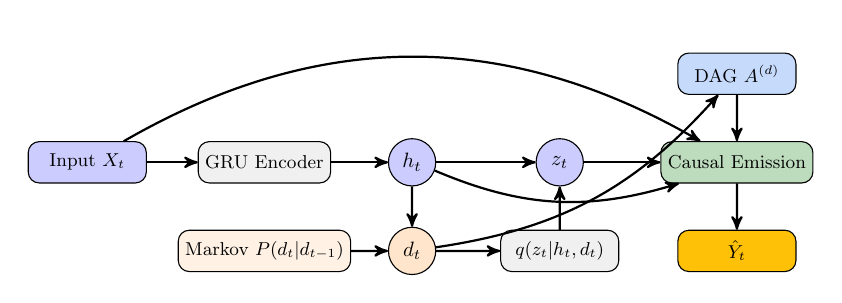
\begin{tikzpicture}[
    scale=0.75,
    transform shape,
    box/.style={rectangle, rounded corners, draw, minimum width=2cm, minimum height=0.7cm, font=\small, fill=lightgray},
    arrow/.style={-{stealth'}, thick},
    latent/.style={circle, draw, minimum size=0.8cm, fill=blue!20},
    regime/.style={circle, draw, minimum size=0.8cm, fill=orange!20}
]
    % Input
    \node[box, fill=blue!20] (input) at (0, 0) {Input $X_t$};
    \node[box] (gru) at (3, 0) {GRU Encoder};
    \node[latent] (h) at (5.5, 0) {$h_t$};

    % Discrete state
    \node[regime] (d) at (5.5, -1.5) {$d_t$};
    \node[box, fill=orange!10] (trans) at (3, -1.5) {Markov $P(d_t|d_{t-1})$};

    % Continuous latent
    \node[latent] (z) at (8, 0) {$z_t$};
    \node[box] (znet) at (8, -1.5) {$q(z_t|h_t,d_t)$};

    % Causal emission
    \node[box, fill=reprogreen!30] (causal) at (11, 0) {Causal Emission};
    \node[box, fill=elecyellow] (pred) at (11, -1.5) {$\hat{Y}_t$};

    % DAG
    \node[box, fill=causalblue!30] (dag) at (11, 1.5) {DAG $A^{(d)}$};

    % Arrows
    \draw[arrow] (input) -- (gru);
    \draw[arrow] (gru) -- (h);
    \draw[arrow] (h) -- (d);
    \draw[arrow] (trans) -- (d);
    \draw[arrow] (h) -- (z);
    \draw[arrow] (d) -- (znet);
    \draw[arrow] (znet) -- (z);
    \draw[arrow] (z) -- (causal);
    \draw[arrow] (h) to[bend right=20] (causal);
    \draw[arrow] (dag) -- (causal);
    \draw[arrow] (d) to[bend right=20] (dag);
    \draw[arrow] (causal) -- (pred);
    \draw[arrow] (input) to[bend left=30] (causal);
\end{tikzpicture}
\end{center}

\vspace{0.2cm}
\textbf{Key Components:}
\begin{itemize}
    \item \textbf{GRU Encoder:} $h_t = \text{GRU}(X_t, Y_{t-1})$ -- captures temporal patterns
    \item \textbf{Discrete State:} $d_t \sim P(d_t | d_{t-1}, h_t)$ -- Markov regime switching
    \item \textbf{Continuous Latent:} $z_t \sim q(z_t | h_t, z_{t-1}, d_t)$ -- within-regime dynamics
    \item \textbf{Causal Emission:} $\hat{Y}_t = \text{ICGNN}(X_t, A^{(d_t)}, h_t, z_t)$ -- FANTOM-style SEM
\end{itemize}
\end{frame}

%==============================================================================
\begin{frame}{Shared vs Independent DAGs}
\textbf{Two Modes for Regime-Specific Graphs:}

\vspace{0.3cm}
\begin{columns}
\begin{column}{0.5\textwidth}
\textbf{1. Independent Mode:}
\begin{itemize}
    \item Separate DAG $A^{(d)}$ per regime
    \item Maximum flexibility
    \item No structural sharing
    \item Best when regimes are very different
\end{itemize}

\vspace{0.2cm}
\begin{equation*}
A^{(d)} = \text{VarDist}_d(A)
\end{equation*}
\end{column}

\begin{column}{0.5\textwidth}
\textbf{2. Shared Backbone Mode:}
\begin{itemize}
    \item Common edges $A_{\text{shared}}$
    \item Plus regime-specific edges $A^{(d)}_{\text{specific}}$
    \item Encourages structural similarity
    \item Better when regimes share core structure
\end{itemize}

\vspace{0.2cm}
\begin{equation*}
A^{(d)} = \sigma(A_{\text{shared}} + A^{(d)}_{\text{specific}})
\end{equation*}
\end{column}
\end{columns}

\vspace{0.3cm}
\textbf{Implementation:}
\begin{itemize}
    \item 3-way categorical for instantaneous edges (i$\to$j, j$\to$i, no edge)
    \item Bernoulli for lagged edges (simpler, no DAG constraint needed)
    \item Gumbel-Softmax for differentiable sampling
\end{itemize}
\end{frame}

%==============================================================================
\begin{frame}{DS3M-Causal: Experimental Results}
\textbf{Multivariate DS3M on QRT Electricity Data:}

\vspace{0.2cm}
\begin{table}
\centering
\small
\begin{tabular}{l|c|c|c|c}
\toprule
\textbf{Country} & \textbf{Spearman} & \textbf{RMSE} & \textbf{Regimes} & \textbf{Samples/Regime} \\
\midrule
\rowcolor{lightgray} Benchmark (Linear) & 0.159 & -- & 1 & -- \\
\midrule
Germany (DE) & \textcolor{warnred}{-0.275} & 0.889 & 2 & 74 / 54 \\
France (FR) & \textcolor{warnred}{-0.087} & 0.952 & 2 & 163 / 7 \\
\textcolor{reprogreen}{\textbf{Joint (ALL)}} & \textcolor{reprogreen}{\textbf{0.408}} & \textbf{0.874} & 2 & 285 / 13 \\
\bottomrule
\end{tabular}
\end{table}

\vspace{0.2cm}
\textbf{Key Observations:}
\begin{itemize}
    \item \textcolor{reprogreen}{Joint model (ALL) achieves Spearman 0.408} -- comparable to FANTOM (0.484)
    \item Country-specific models show negative Spearman -- possible overfitting
    \item Regime detection works: 2 regimes discovered in all cases
    \item \textcolor{warnred}{DS3M-Causal hybrid jobs still running} -- full results pending
\end{itemize}

\vspace{0.2cm}
\textbf{Configuration:} 32 features, $d_{\text{dim}}=2$ regimes, $h_{\text{dim}}=32/48$, 200 epochs
\end{frame}

%==============================================================================
\begin{frame}{DS3M-Causal: Architecture Comparison}
\begin{table}
\centering
\small
\begin{tabular}{l|ccc}
\toprule
\textbf{Feature} & \textbf{DS3M} & \textbf{FANTOM} & \textbf{DS3M-Causal} \\
\midrule
Regime switching & Markov & EM-based & Markov \\
Causal structure & \textcolor{warnred}{\texttimes} & \textcolor{reprogreen}{\checkmark} & \textcolor{reprogreen}{\checkmark} \\
Continuous latent $z_t$ & \textcolor{reprogreen}{\checkmark} & \textcolor{warnred}{\texttimes} & \textcolor{reprogreen}{\checkmark} \\
GRU encoder & \textcolor{reprogreen}{\checkmark} & \textcolor{warnred}{\texttimes} & \textcolor{reprogreen}{\checkmark} \\
DAG constraint & \textcolor{warnred}{\texttimes} & \textcolor{reprogreen}{\checkmark} & \textcolor{reprogreen}{\checkmark} \\
Regime-specific graphs & N/A & \textcolor{reprogreen}{\checkmark} & \textcolor{reprogreen}{\checkmark} \\
Shared backbone option & N/A & \textcolor{warnred}{\texttimes} & \textcolor{reprogreen}{\checkmark} \\
\bottomrule
\end{tabular}
\end{table}

\vspace{0.3cm}
\textbf{Novel Contributions:}
\begin{itemize}
    \item \textbf{First hybrid} combining state-space model with causal discovery
    \item \textbf{Shared backbone} option for structured regime similarity
    \item \textbf{Conditioning on $(h_t, z_t)$} allows dynamic causal effects
    \item \textbf{Full ELBO} with DAG + sparsity + KL terms
\end{itemize}
\end{frame}

%==============================================================================
\begin{frame}{DS3M-Causal: Loss Function}
\textbf{Full ELBO Objective:}
\begin{equation*}
\mathcal{L} = \underbrace{\mathbb{E}_{q(d,z)}[-\log p(Y|X,d,z,A)]}_{\text{Reconstruction (NLL)}} + \underbrace{\lambda_{\text{KL}} \cdot (\text{KL}_d + \text{KL}_z)}_{\text{Latent Regularization}} + \underbrace{\lambda_{\text{DAG}} \cdot h(A)}_{\text{DAG Penalty}} + \underbrace{\lambda_{\text{sparse}} \cdot \|A\|_1}_{\text{Sparsity}}
\end{equation*}

\vspace{0.3cm}
\textbf{Per-Regime Computation:}
\begin{equation*}
\mathcal{L}_t = \sum_{d=1}^{D} \gamma_{t,d} \left[ -\log p(Y_t | X_t, A^{(d)}, h_t, z_t^{(d)}) + \text{KL}(q(z_t^{(d)}) \| p(z_t^{(d)})) \right]
\end{equation*}

where $\gamma_{t,d} = P(d_t = d | h_t, Y_t, d_{t-1})$ is the regime posterior.

\vspace{0.3cm}
\textbf{Training:}
\begin{itemize}
    \item Augmented Lagrangian for DAG constraint (same as FANTOM)
    \item Adam optimizer with gradient clipping
    \item 200 epochs, early stopping on validation loss
\end{itemize}
\end{frame}

%==============================================================================
\section{Future Work}

\begin{frame}{Ongoing \& Planned Work}

\textbf{1. DS3M-Causal Hybrid (In Progress):}
\begin{itemize}
    \item \textcolor{reprogreen}{6 jobs submitted} -- FR/DE/ALL $\times$ independent/shared\_backbone
    \item Waiting for cluster resources (GPU queue)
    \item Will compare shared backbone vs independent DAG modes
\end{itemize}

\vspace{0.2cm}
\textbf{2. Next Steps:}
\begin{enumerate}
    \item \textbf{Causal Effect Module}
    \begin{itemize}
        \item Implement do-calculus interventions
        \item Compute ATEs for key variables
    \end{itemize}

    \item \textbf{Enhanced Regime Detection}
    \begin{itemize}
        \item Analyze regime-specific causal structures
        \item Correlate regimes with known market events
    \end{itemize}

    \item \textbf{Policy Scenario Analysis}
    \begin{itemize}
        \item Simulate renewable expansion scenarios
    \end{itemize}
\end{enumerate}
\end{frame}

%==============================================================================
\begin{frame}{Potential Methodological Contributions}
\textbf{For Publication:}

\vspace{0.3cm}
\textbf{1. Supervised Causal Discovery Framework}
\begin{itemize}
    \item Formalize TARGET constraint methodology
    \item Theoretical analysis of identifiability
    \item Benchmark on multiple domains
\end{itemize}

\vspace{0.3cm}
\textbf{2. Energy Market Causal Analysis}
\begin{itemize}
    \item Comprehensive analysis of DE/FR electricity markets
    \item Regime detection aligned with market events
    \item Policy implications from causal structure
\end{itemize}

\vspace{0.3cm}
\textbf{3. Causal Effect Estimation in Non-Stationary Settings}
\begin{itemize}
    \item Extend FANTOM with intervention capabilities
    \item Handle regime-specific treatment effects
    \item Uncertainty quantification for policy recommendations
\end{itemize}
\end{frame}

%==============================================================================
\begin{frame}{Conclusions}
\textbf{What We've Achieved:}
\begin{itemize}
    \item \textcolor{reprogreen}{Adapted FANTOM for supervised causal discovery}
    \item \textcolor{reprogreen}{Germany: 3x improvement over benchmark (Spearman 0.484 vs 0.159)}
    \item \textcolor{reprogreen}{France: 86\% improvement over benchmark (Spearman 0.296)}
    \item \textcolor{reprogreen}{Discovered interpretable causal structures for both markets}
    \item \textcolor{reprogreen}{Developed DS3M-Causal hybrid} -- combining Markov switching with causal graphs
\end{itemize}

\vspace{0.2cm}
\textbf{Key Insights:}
\begin{itemize}
    \item \textbf{Coal returns} strongest lagged predictor (commodity price impact)
    \item \textbf{Wind power} strongest instantaneous effect (renewable supply)
    \item Joint model (ALL) with DS3M achieves Spearman 0.408
\end{itemize}

\vspace{0.2cm}
\textbf{Contributions:}
\begin{itemize}
    \item Novel supervised causal discovery methodology
    \item \textbf{First hybrid} state-space + causal discovery model
    \item Shared backbone option for structured regime similarity
\end{itemize}
\end{frame}

%==============================================================================
\begin{frame}
\centering
\Huge Thank You

\vspace{1cm}
\Large Questions?

% \vspace{1cm}
% \normalsize
% Code: \texttt{/lustre/home/dthumm/CASTOR/electricity/}

% \vspace{0.3cm}
% Results: \texttt{outputs/germany\_*/metrics.json}
\end{frame}

%==============================================================================
\appendix
\section{Appendix}

\begin{frame}{Appendix: Detailed Literature Review (1/2)}
\textbf{Constraint-Based Causal Discovery:}
\begin{itemize}
    \item \textbf{PC Algorithm} (Spirtes et al., 2000): Tests conditional independencies
    \item \textbf{FCI} (Spirtes et al., 2000): Handles latent confounders
    \item \textbf{PCMCI} (Runge, 2018): Extends PC for time series
    \item \textbf{PCMCI+} (Runge, 2020): Adds contemporaneous discovery
    \item \textcolor{warnred}{Limitation:} Requires faithfulness, no instantaneous in original PCMCI
\end{itemize}

\vspace{0.3cm}
\textbf{Score-Based Methods:}
\begin{itemize}
    \item \textbf{NOTEARS} (Zheng et al., 2018): Continuous DAG optimization
    \item \textbf{DYNOTEARS} (Pamfil et al., 2020): Temporal extension
    \item \textbf{DAG-GNN} (Yu et al., 2019): Graph neural networks for DAGs
    \item \textcolor{warnred}{Limitation:} Linear SEMs, no regime detection
\end{itemize}
\end{frame}

%==============================================================================
\begin{frame}{Appendix: Detailed Literature Review (2/2)}
\textbf{Variational / Deep Learning Methods:}
\begin{itemize}
    \item \textbf{DECI} (Geffner et al., 2022): Variational inference + normalizing flows
    \item \textbf{Rhino} (Gong et al., 2023): History-dependent noise
    \item \textbf{CASTOR} (Huang et al., 2023): Regime-switching temporal causal discovery
    \item \textbf{FANTOM} (Liang et al., 2024): EM-based multi-regime with non-Gaussian
\end{itemize}

\vspace{0.3cm}
\textbf{Electricity Price Modeling:}
\begin{itemize}
    \item \textbf{Traditional:} ARIMA, GARCH for volatility (Weron, 2014)
    \item \textbf{ML:} Random forests, XGBoost, neural networks
    \item \textbf{Regime-switching:} Markov-switching models (Hamilton, 1989)
    \item \textcolor{warnred}{Gap:} No causal discovery for regime-specific price drivers
\end{itemize}

\vspace{0.3cm}
\textbf{Our Contribution:} First to combine \textbf{supervised} causal discovery with \textbf{regime detection} and \textbf{non-Gaussian noise} for electricity markets.
\end{frame}

%==============================================================================
\begin{frame}{Appendix: Technical Details}
\textbf{Prior Network Implementation:}
\begin{itemize}
    \item 2-layer MLP: $t \to \text{Hidden}(32) \to \text{Softmax}(K)$
    \item Input: Normalized time index $t/T \in [0,1]$
    \item Output: $P(\text{regime}=k | t)$ for each $k \in \{1, \ldots, K\}$
    \item \textbf{Purpose:} Learn smooth temporal regime transitions
    \item \textbf{NOT related to instantaneous effects} (those are in $A[0,:,:]$)
\end{itemize}

\vspace{0.1cm}
\textbf{Regime Pruning:}
\begin{itemize}
    \item Threshold: $\zeta = 100$ samples minimum per regime
    \item If $\sum_i \gamma_{ik} < \zeta$, regime $k$ is removed
    \item Prevents overfitting to small data segments
    \item Remaining regime probabilities renormalized
\end{itemize}

\vspace{0.1cm}
\textbf{Collinearity Handling:}
\begin{itemize}
    \item Not explicitly addressed (no VIF filtering)
    \item DAG structure provides implicit handling (one path sufficient)
    \item Sparsity regularization ($\lambda_{\text{sparse}}$) encourages parsimonious solutions
\end{itemize}
\end{frame}

%==============================================================================
\begin{frame}{Appendix: DAG Constraint $h(A)$ Explained}
\textbf{Why is the DAG constraint necessary?}

\vspace{0.2cm}
Without constraints, learned graphs may contain \textbf{cycles} (e.g., $X \to Y \to X$), which:
\begin{itemize}
    \item Violate causal semantics (causes must precede effects)
    \item Make interventional reasoning impossible
    \item Lead to infinite loops in structural equations
\end{itemize}

\vspace{0.3cm}
\textbf{The NOTEARS Constraint (Zheng et al., 2018):}
\begin{equation*}
h(A) = \text{tr}(e^{A \circ A}) - d = 0 \quad \Leftrightarrow \quad A \text{ is acyclic}
\end{equation*}

\vspace{0.2cm}
\textbf{Why does this work?}
\begin{itemize}
    \item $A \circ A$ = element-wise square (ensures non-negative entries)
    \item $e^{A \circ A} = I + (A \circ A) + \frac{(A \circ A)^2}{2!} + \ldots$ counts weighted paths
    \item Diagonal entry $(e^{A \circ A})_{ii}$ counts paths from node $i$ back to itself
    \item If $A$ is a DAG: no cycles $\Rightarrow$ diagonal entries = 1 $\Rightarrow$ $\text{tr}(e^{A \circ A}) = d$
    \item If $A$ has cycles: self-paths exist $\Rightarrow$ $\text{tr}(e^{A \circ A}) > d$
\end{itemize}

\vspace{0.2cm}
\textbf{Key insight:} Continuous relaxation enables gradient-based DAG learning!
\end{frame}

%==============================================================================
\begin{frame}{Appendix: Latent Confounders}
\textbf{Does FANTOM Handle Latent Variables (Unobserved Confounders)?}

\vspace{0.3cm}
\textbf{Short Answer:} No explicit treatment of latent confounders.

\vspace{0.3cm}
\textbf{Assumption:} Causal sufficiency -- all common causes are observed
\begin{itemize}
    \item DECI/FANTOM assumes no hidden confounders between observed variables
    \item This is a standard assumption in score-based causal discovery
    \item Violation can lead to \textbf{spurious edges} in the learned DAG
\end{itemize}

\vspace{0.3cm}
\textbf{Mitigations in Our Setting:}
\begin{itemize}
    \item \textbf{Rich feature set:} 35 variables covering major market drivers
    \item \textbf{Temporal structure:} Lagged effects reduce instantaneous confounding
    \item \textbf{Domain knowledge:} Included all known drivers (weather, production, commodities)
    \item \textbf{Sparsity regularization:} Reduces spurious edges
\end{itemize}

\vspace{0.3cm}
\textbf{Future Work:} Consider methods like FCI or latent variable models if confounding suspected.
\end{frame}

%==============================================================================
\begin{frame}{Appendix: From Causal Discovery to Target Estimation}
\textbf{How We Adapted Causal Discovery for Supervised Prediction:}

\vspace{0.2cm}
\textbf{1. Standard Causal Discovery (FANTOM):}
\begin{itemize}
    \item Learns full DAG $A$ over \textbf{all} variables
    \item Objective: Maximize likelihood $p(X | A, W)$ for all variables
    \item Output: Causal structure among all variables
\end{itemize}

\vspace{0.2cm}
\textbf{2. Our Modification (FANTOMElectricity):}
\begin{itemize}
    \item Add TARGET variable as the \textbf{last node}
    \item Constrain: $A_{[\text{TARGET}, :]} = 0$ (no outgoing edges from TARGET)
    \item Effect: TARGET becomes a \textbf{sink node} -- purely an effect variable
    \item Prediction: Use learned $W_{[:, \text{TARGET}]}$ to estimate TARGET from parents
\end{itemize}

\vspace{0.2cm}
\textbf{3. Key Insight:}
\begin{equation*}
\hat{y}_{\text{TARGET}} = f\left(\sum_{i \in \text{Pa}(\text{TARGET})} W_{i,\text{TARGET}} \cdot X_i\right)
\end{equation*}
\begin{itemize}
    \item The SEM naturally provides predictions via parent-weighted aggregation
    \item Normalizing flow models residual noise $\varepsilon_{\text{TARGET}}$
\end{itemize}
\end{frame}

%==============================================================================
\begin{frame}{Appendix: Prediction Mechanism Details}
\textbf{How Predictions Are Generated:}

\vspace{0.1cm}
\begin{center}
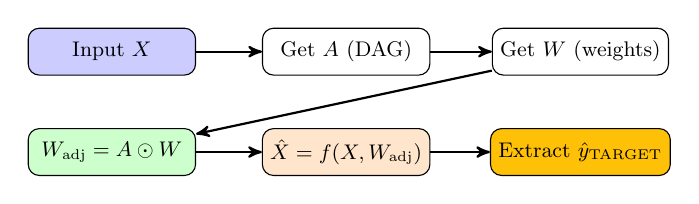
\begin{tikzpicture}[
    scale=0.85,
    transform shape,
    box/.style={rectangle, rounded corners, draw, minimum width=2.5cm, minimum height=0.7cm, font=\small},
    arrow/.style={-{stealth'}, thick}
]
    % Input
    \node[box, fill=blue!20] (input) at (0, 0) {Input $X$};
    \node[box] (adj) at (3.5, 0) {Get $A$ (DAG)};
    \node[box] (weight) at (7, 0) {Get $W$ (weights)};

    % Processing
    \node[box, fill=green!20] (wadj) at (0, -1.5) {$W_{\text{adj}} = A \odot W$};
    \node[box, fill=orange!20] (pred) at (3.5, -1.5) {$\hat{X} = f(X, W_{\text{adj}})$};
    \node[box, fill=elecyellow] (target) at (7, -1.5) {Extract $\hat{y}_{\text{TARGET}}$};

    % Arrows
    \draw[arrow] (input) -- (adj);
    \draw[arrow] (adj) -- (weight);
    \draw[arrow] (weight) -- (wadj);
    \draw[arrow] (wadj) -- (pred);
    \draw[arrow] (pred) -- (target);
\end{tikzpicture}
\end{center}

\vspace{0.1cm}
\textbf{Structural Equation Model (SEM):}
\begin{equation*}
X_j = f_j\left(\sum_{l=0}^{L} \sum_{i=1}^{d} W_{l,i,j} \cdot X_{t-l,i}\right) + \varepsilon_j
\end{equation*}
where $f_j$ is a neural network and $\varepsilon_j \sim$ normalizing flow.

\vspace{0.1cm}
\textbf{For TARGET:}
\begin{itemize}
    \item Only \textbf{incoming edges} contribute (outgoing edges constrained to 0)
    \item Prediction uses both \textbf{instantaneous} ($l=0$) and \textbf{lagged} ($l>0$) parents
    \item Heteroscedastic noise: variance $\sigma^2_{\text{TARGET}}$ also learned
\end{itemize}
\end{frame}

%==============================================================================
\begin{frame}{Appendix: Germany Regime Detection (K=4)}
\textbf{Regime Probability Over Time:}
\begin{center}
\includesvg[width=0.95\textwidth]{figures/de_regime_k4_probability.svg}
\end{center}
\vspace{0.1cm}
\textbf{Result:} 2 regimes discovered (589 + 53 samples). Colors show regime assignment probability.
\end{frame}

%==============================================================================
\begin{frame}{Appendix: Germany Regime Changepoints (K=4)}
\textbf{Detected Changepoints:}
\begin{center}
\includesvg[width=0.95\textwidth]{figures/de_regime_k4_changepoints.svg}
\end{center}
\vspace{0.1cm}
\textbf{Interpretation:} Vertical lines mark regime transitions. Minor regime (53 samples) captures distinct market conditions.
\end{frame}

%==============================================================================
\begin{frame}{Appendix: Germany Time Series with Regimes (K=4)}
\textbf{Feature Time Series Colored by Regime:}
\begin{center}
\includesvg[height=0.8\textheight]{figures/de_regime_k4_timeseries.svg}
\end{center}
\end{frame}

%==============================================================================
\begin{frame}{Appendix: France Regime Detection (K=4)}
\textbf{Regime Probability Over Time:}
\begin{center}
\includesvg[width=0.95\textwidth]{figures/fr_regime_k4_probability.svg}
\end{center}
\vspace{0.1cm}
\textbf{Result:} 2 regimes discovered (744 + 104 samples). Main regime dominates with occasional transitions.
\end{frame}

%==============================================================================
\begin{frame}{Appendix: France Regime Changepoints (K=4)}
\textbf{Detected Changepoints:}
\begin{center}
\includesvg[width=0.95\textwidth]{figures/fr_regime_k4_changepoints.svg}
\end{center}
\vspace{0.1cm}
\textbf{Interpretation:} Minor regime (104 samples) shows \textcolor{reprogreen}{positive CARBON\_RET} as top driver vs negative weights in main regime.
\end{frame}

%==============================================================================
\begin{frame}{Appendix: France Time Series with Regimes (K=4)}
\textbf{Feature Time Series Colored by Regime:}
\begin{center}
\includesvg[width=0.9\textheight]{figures/fr_regime_k4_timeseries.svg}
\end{center}
\end{frame}

\end{document}
